\documentclass{standalone}
\usepackage{tikz}

\usepackage{color}

\usetikzlibrary{arrows.meta}
\usetikzlibrary{calc}
\usetikzlibrary{shapes}
\usetikzlibrary{bending}
\usetikzlibrary{patterns}

\usepackage{gensymb}


\begin{document}
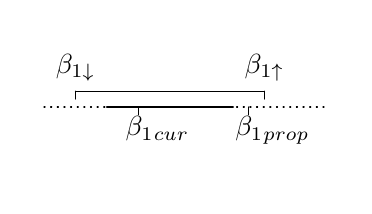
\begin{tikzpicture}[scale=2,cap=round]

\draw [fill=white,white] (0,0) rectangle (2,1); 

\draw[dotted] (0.1,0.5)  -- (1.9, 0.5);
\draw[thick]  (0.5,0.5) -- (1.3, 0.5);

\draw (0.7,0.5) -- (0.7,0.45);

\node[below] at (0.82,0.5) {$\beta_1{_{cur}}$};

\draw (0.3,0.6) -- (1.5,0.6);
\draw (0.3,0.6) -- (0.3, 0.55);
\draw (1.5,0.6) -- (1.5, 0.55);
\node[above] at (0.3,0.6) {$\beta_{1\downarrow}$};
\node[above] at (1.5,0.6) {$\beta_{1\uparrow}$};

\node[below] at (1.55,0.5) {$\beta_1{_{prop}}$};
\draw (1.4,0.5) -- (1.4,0.45);

\end{tikzpicture}
\end{document}